\chapter{Implementation Details}
In this chapter a more in depth explanation of the implementation of the project will be provided. The operations for retrieving the responses (which will be also refered to as \emph{PUFs} from here on) and implementing the challenge-response mechanism are done partly on the host side and partly on the board (synonymous of \emph{device}) side.

The board is responsible for the following operations:
\begin{enumerate}
	\item Read the PUFs from the RAM and store them in the SRAM;
	\item Return the list of all PUFs to the host;
	\item Return a specific PUF corresponding to the challenge sent by the host.
\end{enumerate}

On the contrary, the host is in charge of the following:
\begin{enumerate}
	\item Asking the board to retrieve the list of all PUFs and storing them in a file that will be used as database for future reference;
	\item Challenge the board to retrieve the PUF and a specific address and then compare it with the corresponding one stored in the database.
\end{enumerate}


\section {PUF retrieval and DB initialization}
At the beginning it is necessary to access the RAM as soon as possible to avoid compromising the content and copy the values found into the SRAM so that they can be read later on. To perform this operation there are some things to be done on both host and board side.

\subsection{Host side}

To get the correct data from the RAM that represent the PUFs it is necessary to access the memory immediately after the board's startup and before writing any data to the RAM. Also to an erase of the memory must be done, so before using copying the PUFs into the SRAM a board initialization is performed.

Once this is done the Host works in three stages. One to prepare the parameters to be send to the board, one to get the response from the board and one to access the DB to store the PUFs. All those stages are implemented in the $examples > puf\_db\_init.cpp$ file.

For the request of the PUFs we don't need to send any parameters. In fact we expect only the list that will be provided from the board. So all we need is a variable where we will store the board response.
The actual communication with the board is done through the use of functions implemented in the L1\_security API. There we have provided the $L1GetPUFS$ function, see figure \ref{fig:L1GetPUFS}, that is responsible of transmitting the parameters to the board and receiving the results from the board.


\begin{figure}[h!]
	\vspace{0.5cm}
	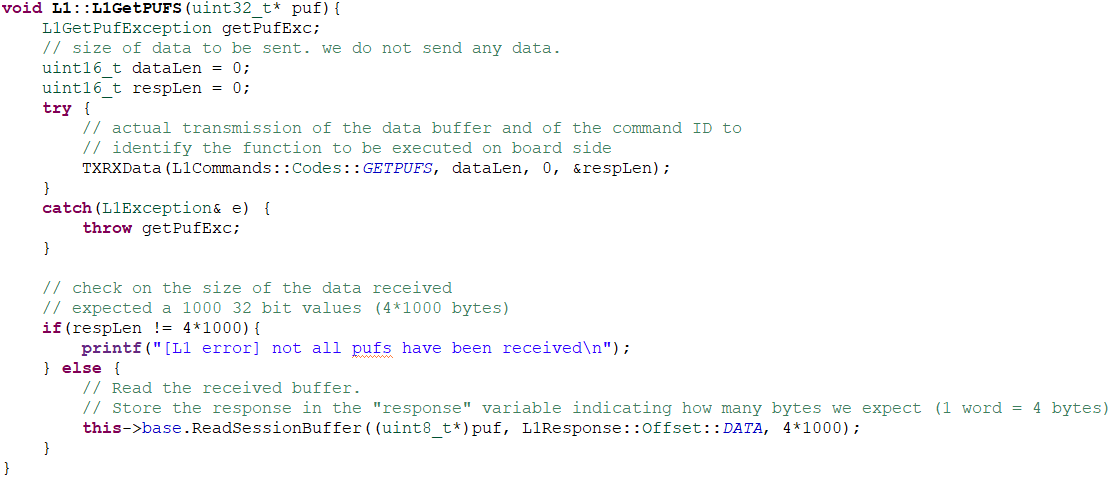
\includegraphics[width = 0.8\textwidth]{images/L1GetPUFS.png}
	\caption{Function responsible for the communicating with the board and receiving the list of PUFs. }
	\label{fig:L1GetPUFS}
\end{figure}

In that piece of code we can see that we are expecting 1000 PUFs. In that operation we must provide the size of the data we are transmitting/receiving and also the ID of the command to be executed on the board side. The response then will be given through a buffer from which we can indicate where to store the result and the amount of bytes the result is composed of. Then the host is responsible of writing that data to the DB.

\subsection{Board side}

In this stage the board is responsible of retrieving the initial data, PUFs, from the RAM and store them to the SRAM so that they can be accessed safely later.

Since the content of the RAM will be overwritten, the PUFs must be copied as soon as possible. For this reason this operation has to be done before any memory initialization. So this operation is done in the startup assembly code in which the reset handler can be found. This way we guarantee that we read the RAM before any memory initialization that could result in compromising the PUFs.

Since the flash needs control registers to be set in order to be accessed in a safe way we relied on the HAL functions provided by STMicroelectronics. More precisely the functions to unlock and program/write in memory. The code written to perform this operation can be seen in figure \ref{fig:code_assembly}

\begin{figure}[h!]
	\centering
	\vspace{0.5cm}
	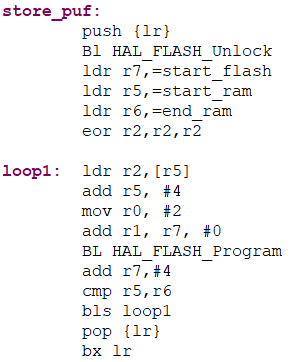
\includegraphics[width = 0.3\textwidth]{images/code_assembly.png}
	\caption{Assembly code to store PUFs into the flash memory. }
	\label{fig:code_assembly}
\end{figure}

Using the reference manual for the MCU (STM32f429) we know the memory mapping of both the SRAM(0x020000000 -  0x02002FFFF) and flash memory(0x08000000 - 0x081FFFFF). Starting from that we scanned the SRAM and loaded the content to a part of the flash that will not overwrite sensible data.

At the end of the execution of the assembly code we expect 1000 PUFs to be stored in the flash memory which will be accessible once we enter the main and eventually the execution loop. At that point we can call the implemented functions and access the content of the SRAM.

Once we have the PUFs in memory we need access to them. This is done in the $puf\_retreive()$ function, found in the $se3\_dispatcher\_core.c$ file. This is the function associated to the command code transmitted from the Host side to the board.

To make the command call possible it is necessary to define these commands in the $se3\_dispatcher\_core.h$ which must reflect the ID associated to the same command also on the host side.

\begin{figure}[h!]
	\vspace{0.5cm}
	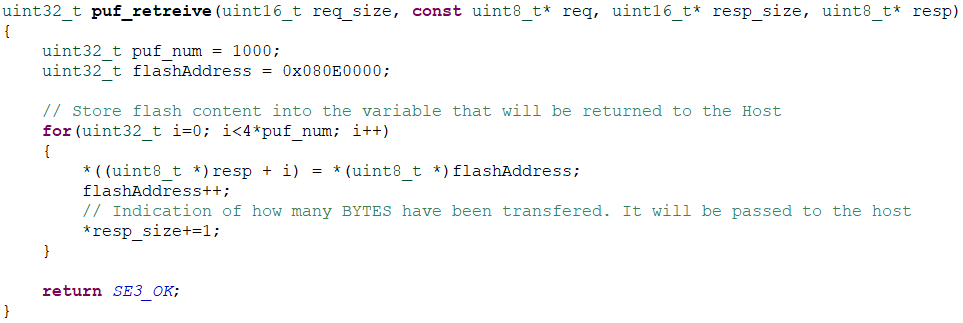
\includegraphics[width = 0.8\textwidth]{images/puf_retreive.png}
	\caption{puf\_retreive function. }
	\label{fig:puf_retreive}
\end{figure}

In the $puf\_retreive()$ function we simply read from the SRAM the PUFS that we stored in the assembly code. This data is the data that will be sent to the host side.


\section {Application of a challenge and verification of the device} 
\label{section:impl_host}

Once we have the DB filled with the PUFs we can use that to check the authenticity of the board by comparing the PUFs in the DB to the ones regenerated by the board. Again to realize the functionality we will have to do some things on the host and some on the board side.

\subsection{Host side}

The approach is similar to the one used for reading the PUFs but now we have different parameters to transmit. In fact we need to provide some data, the challenge, for the board to work on. So the Host is responsible of getting the challenge, use it to access the DB and retrieve the expected response, PUF. Then the challenge is sent to the board expecting in return the actual response to that challenge.

Then the next stage is to perform the actual transmit/receive which is done using in the L1ChallengePUF function of the L1 API, shown in figure \ref{fig:L1ChallengePUF}.

\begin{figure}[h!]
	\vspace{0.5cm}
	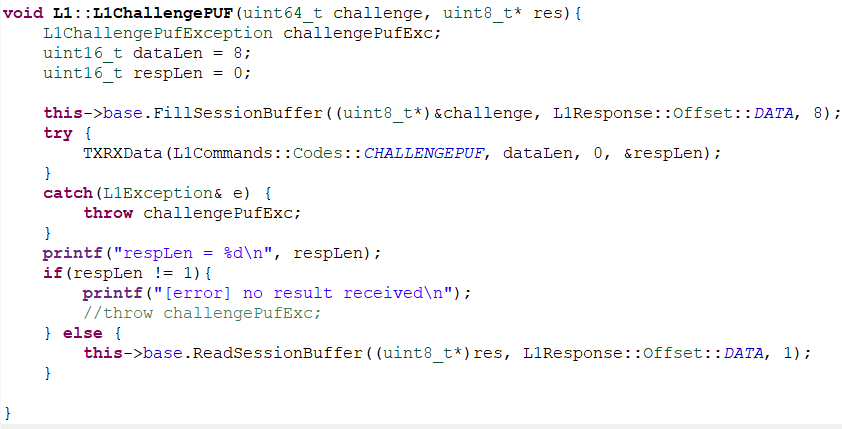
\includegraphics[width = 0.8\textwidth]{images/L1ChallengePUF.png}
	\caption{L1ChallengePUF function for transmitting challenge and response PUF}
	\label{fig:L1ChallengePUF}
\end{figure}


In this function we have some data to transmit and the TXRX works with bytes we have to provide the size of the data to be sent/received in bytes which is 4 since we transmit just 32bit of the challenge. Then as response we expect just one PUF so another 4 bytes.

Once the Host has both expected and actual response it compares them using an acceptable Hamming distance. The one chosen is a Hamming distance of 4 based on statistical results. These operations are done in the $examples > puf\_challenge.cpp$ file shown in figure \ref{fig:puf_challenge.cpp}

\begin{figure}[h!]
	\vspace{0.5cm}
	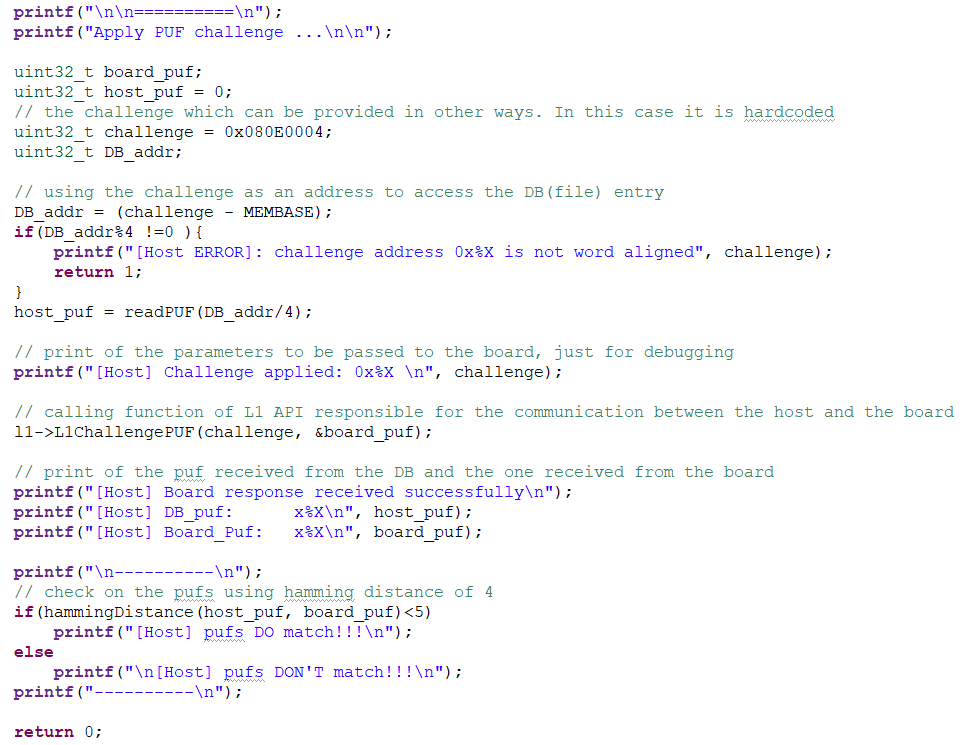
\includegraphics[width = 0.8\textwidth]{images/puf_challenge.png}
	\caption{puf\_challenge.cpp}
	\label{fig:puf_challenge.cpp}
\end{figure}

\subsection{Board side}

The Board at this point has been provided with the challenge. This data has been sent using Little endian encoding so before being able to use the parameter passed a reconstruction is needed.

So we extract the compacted data received and obtain the challenge. From there we can access the SRAM using the challenge as an address. This will be the actual PUF returned to the Host.

\begin{figure}[h!]
	\vspace{0.5cm}
	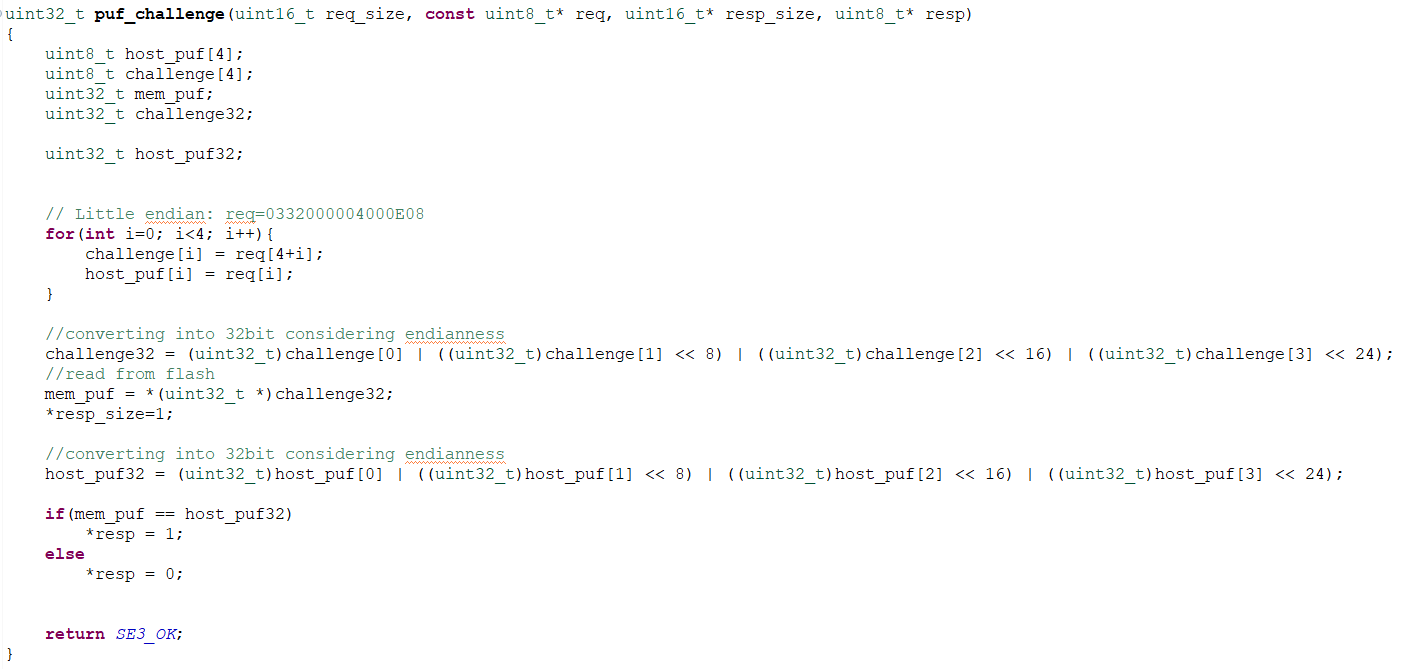
\includegraphics[width = 0.8\textwidth]{images/puf_challenge_board.png}
	\caption{puf\_challenge\_board function on the board side}
	\label{fig:puf_challenge_board}
\end{figure}
